\documentclass[12pt,a4paper]{article}
\usepackage[utf8]{inputenc}
\usepackage[T1]{fontenc}
\usepackage{amsmath, amsfonts, amssymb}

%\usepackage{pdfpages}


%Import graphs
\usepackage{graphicx}
\usepackage{caption,subcaption}
\usepackage[section]{placeins}
\usepackage{float}
\usepackage{multicol}
\usepackage{makecell}
\usepackage{adjustbox}

%color for headings
\usepackage{sectsty}
\chapterfont{\color{YellowOrange}}  % sets colour of chapters
\allsectionsfont{\color{green!5!orange!90!}}  % sets colour of sections
%\captionsetup[figure]{labelfont={color=cyan}}
\captionsetup{labelfont={color=cyan}}

\newcommand\blankpage{%
	\null
	\thispagestyle{empty}%
	\addtocounter{page}{-1}%
	\newpage}
%\usepackage{chngcntr} %counter in appendix
%TOC BACKGROUND COLOR
\usepackage{tcolorbox}

%Bibliography style
%\usepackage[square,numbers]{natbib} %% Own document-numbered style

\usepackage{natbib} %% For MSc Thesis

\graphicspath{{gfx/}}
\usepackage[title]{appendix}

\usepackage[hidelinks]{hyperref}
\usepackage{tocbibind}

%\includeonly{frontmatter/titlenew} %mainmatter/results, frontmatter/abstract, mainmatter/numerics, mainmatter/introduction

%PARAGRAPH SETTINGS
\setlength{\parindent}{12pt}
\numberwithin{equation}{section}
\usepackage{array}
%\usepackage[table]{xcolor} % Highlight table row


\begin{document}
	

\begin{titlepage}
	
	\begin{center}
		{\LARGE University of Cambridge}\\[1.5cm]
		{\Large Department of Engineering}\\[1.5cm]
		
		
		
\includegraphics[scale=0.5]{logo.jpg}\\[1.618cm]
		
		%\linespread{2.0}
		
		\huge {\bfseries Progress Report 0}\\[2cm]
		%\linespread{1}
		{\Large\bf Ekrem Ekici}\\[0.5cm]
		{\large\bf PhD in Engineering}\\[1.618cm]
		{\large \emph{Supervisor:} Prof Matthew Juniper}\\[0.5cm]
		%\vspace{\fill}
		{\large\bf January 4, 2021}
		
	\end{center}
\newpage
\end{titlepage}

%\begin{titlepage}
	
	\begin{center}
		{\color{white}
			{\LARGE University of Birmingham}\\[0.25cm]
			{\Large School of Mechanical Engineering}\\[1.5cm]
			\linespread{1.2}\huge {\bfseries Design and Simulation of Converging Diverging Supersonic Nozzle}\\[1.5cm]
			
			
\includegraphics[scale=0.07]{logo.png}
			
			
			\linespread{1}
			{\Large\bf Ekrem Ekici}\\[0.5cm]
			{\large\bf MSc Advanced Mechanical Engineering}\\[0.5cm]
			{\large \emph{Supervisor:} Dr Jason Stafford}\\[0.5cm]
			%\vspace{\fill}
			{\large\bf September 4, 2020}
		}
	\end{center}
	\pagecolor{black}\afterpage{\nopagecolor}
	\afterpage{\blankpage}
\end{titlepage}

%\begin{titlepage}
	
	\begin{center}
		{\Large \textbf{University of Birmingham}}\\[0.25cm]
		{\Large College of Engineering and Physical Sciences}\\[0.5cm]
		%\linespread{1.2}\huge {\bfseries Design and Simulation of Converging Diverging Supersonic Nozzle}\\[1.5cm]
		{\Large \textbf{Department of Mechanical Engineering}}\\[0.25cm]
		{\Large School of Engineering}\\[0.5cm]
		
\includegraphics[scale=0.04]{logo.png}\\[0.5cm]
		\linespread{1}
		{\LARGE MSc Advanced Mechanical Engineering}\\[1.25cm]
		{\LARGE \textbf{Advanced Project}}\\[1.25cm]
		{\Large\bf 2019-20 Session}\\[1.25cm]		
		{\LARGE\bf FINAL REPORT}\\[0.75cm]
	\end{center}
	\FloatBarrier
	\begin{table}[htb!]
		\begin{tabular}{ll}
			{\Large Surname}    & {\Large \textbf{Ekici}}              \\[3ex]
			{\Large First Name} & {\Large \textbf{Ekrem}}              \\[3ex]
			{\Large ID Number}  & {\Large \textbf{2104821}}            \\[3ex]
			{\Large Supervisor's Name} & {\Large \textbf{Dr Jason Stafford}}          \\[3ex]
			{\Large Project Title}     & {\Large \textbf{Design and Simulation of Converging}}\\[1.5ex]
			     & {\Large \textbf{Diverging Supersonic Nozzle}}\\
		\end{tabular}
	\end{table}
	\FloatBarrier
	\afterpage{\blankpage}
\end{titlepage}


%{\Large Surname}				{\Large\bf         Ekici}\\[0.25cm]
%{\Large First Name}             {\Large\bf Ekrem }\\[0.25cm]
%{\Large ID Number} 		     	{\Large\bf 2104821}\\[0.25cm]
%{\Large Supervisor's Name}       {\Large\bf Dr Jason Stafford}\\[0.25cm]
%{\Large Project Title}       {\Large\bf Design and Simulation of Converging Diverging Supersonic Nozzle }
\pagenumbering{roman}
%
\cleardoublepage
\phantomsection
\begin{center}
	\section*{Abstract}
	\addcontentsline{toc}{section}{\numberline{}Abstract}%
\end{center}

The recent demand for commercial sub-orbital and orbital flight has increased the prevalence of supersonic propulsion. A key component of this in rocket engines is the converging-diverging nozzle which accelerates combustion gases to supersonic speeds to deliver the thrust required during lift-off and flight. The shape of this nozzle influences the flow conditions and must be properly designed to provide the maximum thrust in a nozzle body with the lowest weight. 

In this thesis, flow in converging-diverging nozzles has been taken into account. One dimensional isentropic flow is analyzed by developing a custom programming library. For two dimensional analysis, the method of characteristics is utilized to obtain shock-free, minimum length wall contour for the diverging section of a supersonic nozzle. This optimal wall contour has been simulated in OpenFOAM finite volume code and a compressible flow solver. Comparative analysis is showed good agreement between method of characteristics and OpenFOAM simulations considering Mach number and temperature distributions of the diverging part. Proposed approaches, developed and implemented using open-source tools, provide a trustworthy solution for predicting the optimal nozzle design and internal flow behaviour under supersonic conditions. 

\afterpage{\blankpage}


%\cleardoublepage
\phantomsection
\section*{Acknowledgements}
\addcontentsline{toc}{section}{\numberline{}Acknowledgements}

 First and foremost, I would like to thank my Allah, who is the most merciful and most compassionate. Without his help and mercy, I was not able to succeed my studies, my journey.\\

 \noindent I would like to continue by thanking my supervisor Dr Jason Stafford for his mentorship and his sincerity.\\
 
 \noindent I would also like to extend my thanks to Turkish government. Without their support and trust, these studies would not be possible. 	\\
 
 \noindent I would also like to express my big thanks to my friends of Ahmet Alperen Koç and Tuğberk Hakan Çetin for their encouragements and supports during my life regardless of good or bad day.\\
 
 \noindent I would also like to convey my thanks to Usamah Choudhary who helped me to overcome the difficulties during my first year in foreign country.\\
 
 \noindent Finally, I would like to say my big appreciations for my dad, mum, brother and sister to fulfil my dreams through this challenging period.\\
 
 \noindent Ekrem Ekici\\
 
 \noindent UoB 04-Sep-2020\\
 \afterpage{\blankpage}

\pagenumbering{arabic}

\begin{tcolorbox}[colback=green!5,arc=5pt,opacityframe=0]
	\tableofcontents
\end{tcolorbox}
%\cleardoublepage
\phantomsection
%\tableofcontents
\section{Motivation}
 
  Over the last five decades the requirement for supersonic and hypersonic propulsion has grown considerably. Prediction of thermoacoustic oscillations gained importance in order to run rocket engines and gas turbines properly. This motivation requires to being capable of solving complicated mathematical models by utilizing adjoint methods.
  
  \section{Mathematical Model}
  
  1D thermoacoustic model has been considered. Mean flow has been set to zero. As can be seen in Figure \ref{fig:model}, open ended elongated tube from 0 to X containing gas at following parameters;
  \begin{itemize}
	\item{Uniform density, $\overline{\rho}$}
	\item{Uniform pressure, $\overline{p}$}
	\item{Ratio of specific heats, $\gamma$}
	\item{Velocity, $u$}
	\item{Pressure, $p$}  
\end{itemize}  
\begin{figure}[!htb]
	
	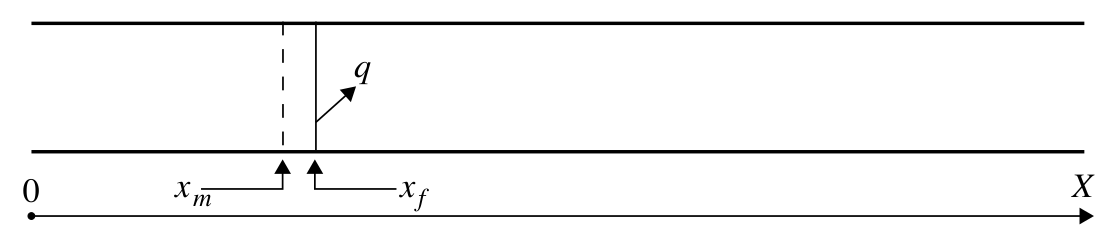
\includegraphics[width=\textwidth]{model.png}
	\caption{Diagram of the open-ended tube extending from 0 (upstream) to X (downstream). The heat
		release, q, occurs at position x f and is a function of the acoustic velocity at x m . The mean flow,
		which is defined as positive in the positive x-direction, is set to zero.}
	\label{fig:model}
	
\end{figure}

%\pagebreak
  





\subsection{Governing Equations}

The 1D acoustic energy and momentum equations are;

\begin{equation}
\overline{\rho}\frac{\partial u}{\partial t}+
\frac{\partial p}{\partial x}=0
\end{equation}

\begin{equation}
\frac{\partial p}{\partial t}+
\gamma \overline{p} \frac{\partial u}{\partial x}=(\gamma-1)q\delta_D (x-x_f)
\end{equation}
  
  
  
  Heat release rate $q(t)=nu(x_m,t_\tau) [W/m^2] $ is placed at $x=x_f$, where $n [J/m^3]$ is a real constant, $\tau$ is time delay, $x_m$ is the measurement position of $u$. Mean
  density drop across the heat source, viscous and thermal dissipations have been neglected. 
  
  $\delta$ is the Dirac delta. Reference length, reference speed and reference pressure are defined as $L_{ref}=X$, $U_{ref}=\overline{c}$ and $P_{ref}=\overline{p}$, respectively.Dimensionless acoustic energy and momentum equations are stated as follows;
  
  \begin{equation}
  \gamma \frac{\partial u}{\partial t}+
  \frac{\partial p}{\partial x}=0
  \label{eq:nondim1}
  \end{equation}
  
  \begin{equation}
  \frac{\partial p}{\partial t}+
  \gamma \frac{\partial u}{\partial x}=(\gamma-1)q\delta_D (x-x_f)
  \label{eq:nondim2}
  \end{equation}
  

\cleardoublepage
\phantomsection
\section{Numerical Methods}


Solution of fluid flow domain has a complex physical and mathematical examinations. 4 methods are commonly preferred to approximate exact solutions of governing  equations. These methods are;
\begin{itemize}
	\item Traveling Wave Method
	\item Helmholtz Finite Difference Method
	\item Helmholtz Finite Element Method
	\item Galerkin Method
\end{itemize}

Each method has been used to solve thermoacoustic governing equations mentioned in previous section. Equation \ref{eq:nondim1} and \ref{eq:nondim2} are determined by applying these methods.


%\pagebreak
\section{Codework}

In order to solve the thermoacoustic governing equations, these 4 method could be programmed to get parametric and quick results. 

JULIA programming language is preferred to perform codeworks.

\subsection{Why Julia Programming Language?}

Julia programming language is developed in order to perform matrix calculations reasonably fast and easy. It is completely open source programming language which enables to work without getting licence. Additionally, having high-level programming syntax makes it easy to learn and its computing performance is blazing fast comparing to programming languages like MATLAB and Python. Furthermore, dynamic type syntax is not requiring to define parameter type(\textit{int, float, double, string, char}) such as fast programming languages C++ and Fortran. 

\subsection{Programming Methodology}

During the code development, mathematical model is created based on object oriented programming technique. Followed methodology is illustrated in Figure \ref{fig:flowchart}. 

\FloatBarrier
\begin{figure}[!t]
	
	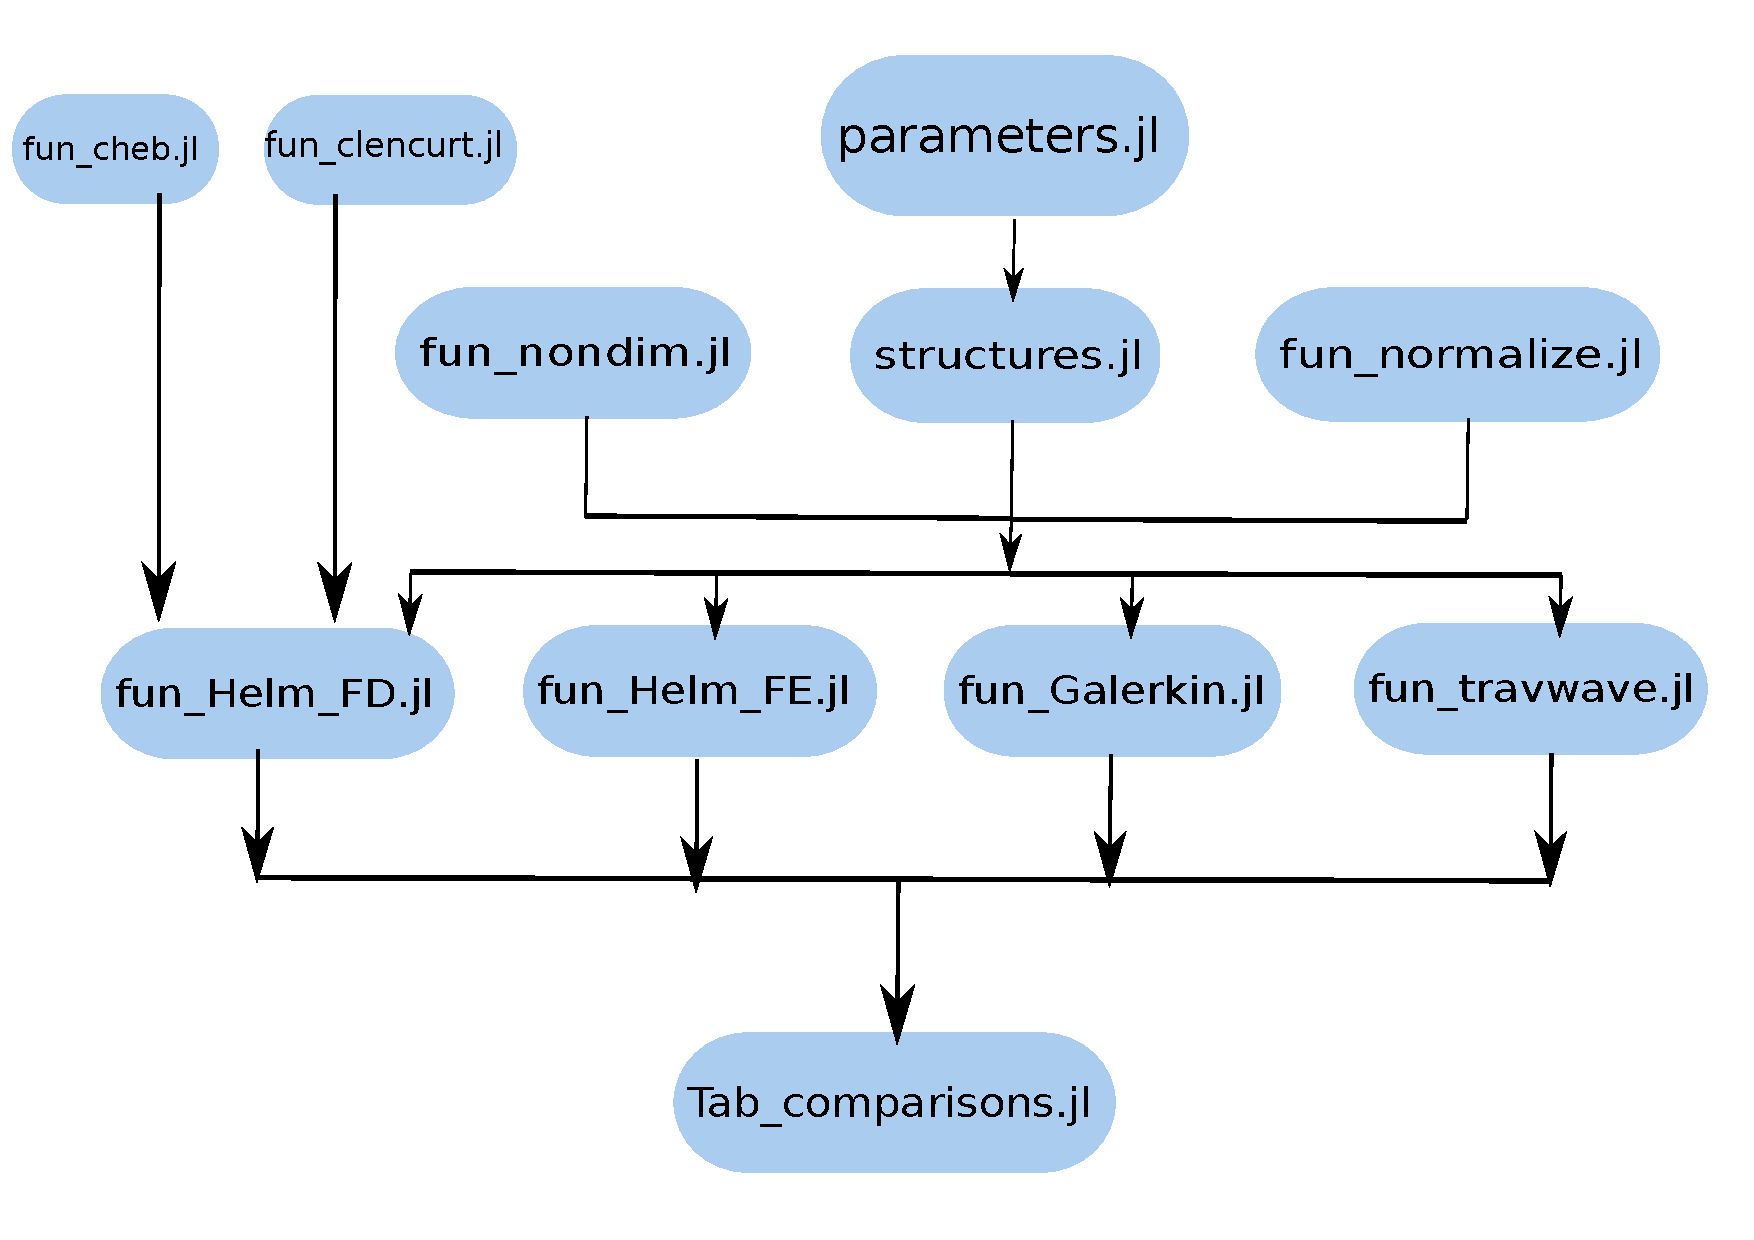
\includegraphics[width=\textwidth]{flowchart.pdf}
	\caption{Codework layout and proposed flowchart}
	\label{fig:flowchart}
	
\end{figure}
\FloatBarrier

Figure \ref{fig:flowchart} shows that each Julia file is connected by following systematic approach. By using these codes, all the methods' calculations can be performed and obtained results and table can be generated in file \textit{Tab\_comparisons.jl}. Script \textit{structures.jl} includes structures of \textbf{emode} and \textbf{ds}. These 2 structures are determined and returned by 4 main scripts;\textit{fun\_Helm\_FD.jl}, \textit{fun\_Helm\_FE.jl}, \textit{fun\_Galerkin.jl and \textit{fun\_travwave.jl}} Specified model parameters are inserted into \textit{parameters.jl} file. Moreover, normalization and non-dimensionalization are performed by \textit{fun\_normalize.jl} and \textit{fun\_nondim.jl} files respectively.

\phantomsection

\section{Results}

Table \ref{tab:eig} shows the eigenvalues, s, determined according to four different
methods for N=400. Figure \ref{fig:plot400} shows the corresponding P (x) and U (x) eigenvectors for the highest
resolution case of each method. The eigenvectors differ only around the heat release zone, at $x = x_f = 0.25$. Main difference coming out in Galerkin method, rest of the three method showed good agreement.

\pagebreak

\begin{table}[]
	\caption{Eigenvalues, s, calculated with four different methods and, where relevant,
		up to five different resolutions, N , for the same thermoacoustic system. The growth
		rate is s r and the frequency is s i . The solutions approach each other as the resolution
		increases. (Tab comparisons.jl)}
	
	\begin{adjustbox}{width=\textwidth,center}
	\begin{tabular}{c c c c c}
		\hline \\ 
		\multicolumn{1}{c}{\textbf{N}} & \textbf{fun\_travwave}                                         & \multicolumn{1}{c}{\textbf{fun\_Helm\_FD}} & \multicolumn{1}{c}{\textbf{fun\_Helm\_FE}}   & \multicolumn{1}{c}{\textbf{fun\_Galerkin}}  \\ [3.2ex]  
		1                              & \multicolumn{1}{l}{\makecell{0.12187530859257883 \\+ 3.2227814041928715im}} & \multicolumn{1}{c}{-}                      & \multicolumn{1}{c}{-}                        & \multicolumn{1}{c}{-}                       \\ [3.2ex]
		10                             & \textbf{-}                                                     & {\makecell{0.12301472009722814 \\+ 3.2222551623591285im}} & {\makecell{1.2649666277747205e-10 \\+ 3.141592631034653im}} & {\makecell{3.42049450595866e-21 \\+ 3.1545273778453238im}} \\ [3.2ex] 
		40                             & \textbf{-}                                                     & {\makecell{0.12363155192096682 \\+ 3.221964689943754im}}  & {\makecell{0.06990252109480179 \\+ 3.184618956384646im}}    & {\makecell{0.1045690701269305 \\+ 3.2100253033952892im}}   \\ [3.2ex] 
		100                            & \textbf{-}                                                     & {\makecell{0.12115229273097906 \\+ 3.2231040481839406im}} & {\makecell{0.12302841468171331 \\+ 3.2235632383934383im}}   & {\makecell{0.12181433836201444 \\+ 3.2228598981240886im}}  \\ [3.2ex] 
		400                            & -                                                              & 
		{\makecell{0.12205739886178892 \\+ 3.2226989128574868im}} & {\makecell{0.12181867950887351 \\+ 3.2227425705073545im}}   & {\makecell{0.12181840527018106 \\+ 3.2227499047678436im}}  \\ [3.2ex]  \hline
	\end{tabular}
\end{adjustbox}


\label{tab:eig}
\end{table}


Table \ref{tab:sens} tabulates the calculated base sensitivities of each method.

\FloatBarrier
\begin{figure}[!t]
	
	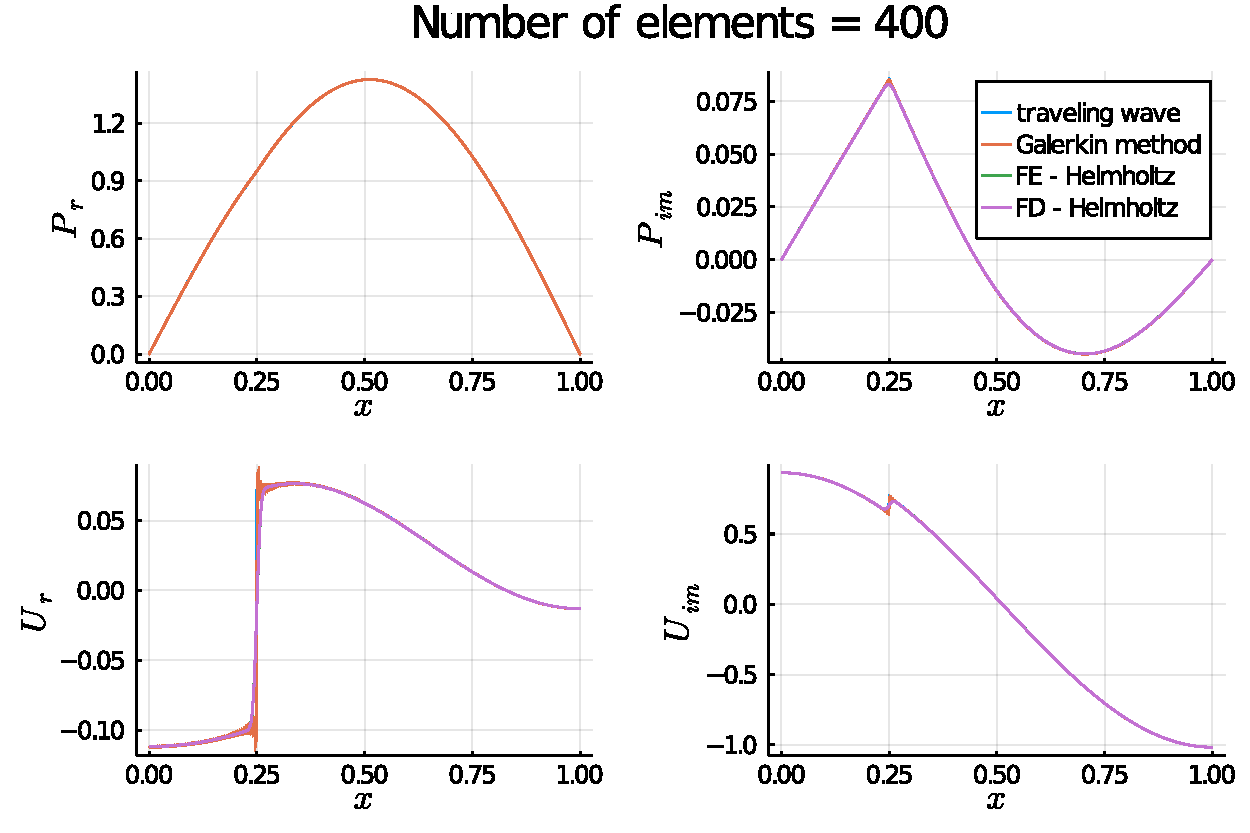
\includegraphics[width=\textwidth]{400plot.pdf}
	\caption{Real and imaginary components of the pressure, P (x), and velocity, U (x), eigenfunctions
		calculated for the highest resolution cases of the methods shown in table 1.  (Tab\_comparisons.jl)}
	\label{fig:plot400}
	
\end{figure}
\FloatBarrier

\pagebreak

\FloatBarrier
\begin{table}[ht!]
	\caption{Base state sensitivities calculated by means of four methods with N = 400 (Tab comparisons.jl)}
	\begin{adjustbox}{width=\textwidth,center}
		\begin{tabular}{lcccc}
			\hline \\ 
			\textbf{}                 & \textbf{$\partial s/\partial n$}                              & \textbf{$\partial s/\partial \tau$}                             & \textbf{$\partial s/\partial x_m$}                            & \textbf{$\partial s/\partial x_f$}                           \\ [3.2ex]
			\textbf{fun\_travwave.jl} & {\makecell{0.10298315656272834 \\+ 0.08269441085108045im}} & {\makecell{0.2539549055356268 \\- 0.34197060875680085im}} & {\makecell{-0.2664856896104548 \\- 0.17766984877202488im}}  & {\makecell{0.43129016791308405 \\+ 0.21134136333692508im}} \\ [3.2ex]
			\textbf{fun\_Helm\_FD.jl} & {\makecell{0.1029381172495191 \\+ 0.08265540766612185im}}  & {\makecell{0.2538373154537853 \\- 0.341812025204056im}}   & {\makecell{-0.2663486625117436 \\- 0.17759310185260918im}}  & {\makecell{0.4310431667740005 \\+ 0.2112708145173602im}}   \\ [3.2ex]
			\textbf{fun\_Helm\_FE.jl} & {\makecell{0.10293804348656137 \\+ 0.08265471643133453im}} & {\makecell{0.2538357312085307 \\- 0.34181243558702773im}} & {\makecell{-0.2663469127817901 \\- 0.17759196026029755im}}  & {\makecell{0.4310398326117469 \\+ 0.21126935565722768im}}  \\ [3.2ex]
			\textbf{fun\_Galerkin.jl} & {\makecell{0.1033169131009024 \\+ 0.08257175330986924im}}  & {\makecell{0.253493305952927 \\- 0.3430377969585296im}}   & {\makecell{-0.26685205730784367 \\- 0.17749521966955883im}} & {\makecell{0.398800858731003 \\+ 0.2259008693655126im}} \\ [3.2ex]  \hline   
		\end{tabular}
	\end{adjustbox}
\label{tab:sens}
\end{table}
\FloatBarrier



%\cleardoublepage
\phantomsection
\section{Conclusion and Future Work}

Supersonic nozzle design by different numeric approximations have been investigated in this study. Firstly, quasi-one dimensional fluid flow analysis of case study has been carried out. Useful one dimensional compressible flow library is developed in Python programming language. Therefore, supersonic flow domain is considered as two dimensional compressible flow and Prandtl-Meyer expansion waves are discussed. Method of characteristics is enabled to find out wall coordinates of supersonic section of rocket nozzle. Each characteristic lines combined with parameters of expansion waves such as Prandtl-Meyer angle, Mach number and Mach angle at certain points in two dimensional domain. Similarly, Python programming language was used to program the method of characteristics.

Generated wall points that obtained by method of characteristics have exported to open-source mesh software Salome to split domain into small grids. Then, meshed geometry is exported to finite volume code to perform computational fluid dynamics analysis. rhoPimpleFoam was utilized as a solver in OpenFOAM open-source framework.
Obtained results indicated that Mach number and temperature distributions along supersonic section are consistent by applying both method of characteristics and computational fluid dynamics.

Taken together, these findings suggest the application of method of characteristics and computational fluid dynamics to  observe supersonic nozzle flow along rocket nozzle. In spite of the fact that quasi-one dimensional analysis can explain only cross-sectional information, method of characteristics is demonstrated its robust approach to determine nozzle length. In addition to this, computational fluid dynamics analysis confirmed this approach by getting similar contours.

Future work will concentrate on the following topics;
\begin{itemize}
	\item Potential shock waves along supersonic flow domain will be considered in OpenFOAM simulations.
	\item Combustion chamber of such a nozzle will be designed and computational fluid dynamics analysis will be performed.
	\item One dimensional Python library will be extended to two dimensional compressible flow by consisting of Prandtl-Meyer expansion wave theory.
	\item More realistic approximations will be made at exit of the nozzle to better understanding of the complex phenomena behind shock waves (such diamond diamond shocks).
	\item Density based compressible flow solver rhoCentralFoam simulations will be stabilized. This solver originally designed to investigate high speed compressible flows and strong shock waves. Hence, it gives more accurate results than pressure-based solvers (rhoSimpleFoam, rhoPimpleFoam).
	\item Nozzle design graphical user interface will be developed in Java programming language.
	\item High speed flows are generally turbulent. So that turbulence models will be considered for further simulations. These results can demonstrate trustworthy roadmap to manufacture rocket nozzles.
\end{itemize} 




%\bibliographystyle{plainnat}  %% Own document-numbered style
\bibliographystyle{apalike}    %% For MSc Thesis
%\bibliographystyle{agsm} %% Harvard Reference Style

%\bibliography{mybib1}
%\cleardoublepage
\phantomsection
%\addcontentsline{toc}{section}{References}






%\cleardoublepage
\phantomsection
\addcontentsline{toc}{section}{Appendix}
\begin{appendices}

\section{Nomenclature}

\noindent $Ma$ : Mach number

\noindent $\alpha$ : speed of sound ($\frac{m}{s}$)

\noindent $k$ : specific heat ratio

\noindent $R$ : specific gas constant ($\frac{J}{kg.K}$)

\noindent $T$ : temperature (K)

\noindent $T_0$ : stagnation temperature (K) 

\noindent $P$ : pressure (Pa)

\noindent $P_0$ : stagnation pressure (Pa) 

\noindent $\rho$ : density ($\frac{kg}{m^3}$)

\noindent $\rho_0$ : stagnation density ($\frac{kg}{m^3}$) 

\noindent $V$ : velocity ($\frac{m}{s}$)

\noindent $A$ : area ($m^2$)

\noindent $A^*$ : critical throat area ($m^2$)

\noindent $\phi$ : velocity potential

\noindent $\theta$ : deflection angle

\noindent $\nu$ : Prandtl-Meyer angle

\noindent $\mu$ : Mach angle

\noindent $\Psi$ : any scalar property
\afterpage{\blankpage}
\newpage

\renewcommand{\thefigure}{A.\arabic{figure}}
\setcounter{figure}{0}
\section{Method of Characteristics Procedure}

In this appendix, method of characteristics procedure is explained step by step by considered supersonic nozzle in this study. Expansion waves are assumed as symmetric according to x axis, then calculations has been made for upper half of the nozzle.

\FloatBarrier
\begin{figure}[!htb]
	\centering
	\includegraphics[scale=0.30]{a1.png}
	\caption{Mach number profile}	

\end{figure}
\FloatBarrier

\noindent {\LARGE \textbf{Tutorial Case}}\\

\noindent Exit Mach number is considered as 2.4 and number of characteristics has taken as N=7. Numbered intersection points, wall points and axis points can be seen in Figure \ref{fig:a2}.

\FloatBarrier
\begin{figure}[!htb]
	\centering
	\includegraphics[scale=0.35]{a2.png}
	\caption{Numbered nozzle profile}	
	\label{fig:a2}
\end{figure}
\FloatBarrier

\pagebreak

\FloatBarrier
\begin{figure}[!htb]
	\centering
	\includegraphics[scale=0.4]{a3.png}
	\caption{Nozzle profile}	
	\label{fig:a3}
\end{figure}
\FloatBarrier

Prandtl-Meyer(PM) angle at the exit for Mach number 2.4;

 $\nu_e = 36.746$

$cd$ characteristic line has same stream properties; 

$\nu_e = \nu_c = 36.746$

Downstream of $cd$ characteristic line is parallel to the x-axis; 

$\theta_e = \theta_c = 0$

Right running characteristic on point $c$ ; 

$K_c^- = \theta_c + \nu_e = 36.746$

Point $c$ and point $a$ on same characteristic $ac$;

$K_c^- = K_a^- = 36.746$

Occurred PM expansion waves of corner $a$;

$\nu_a = \nu(1)+\Delta\theta$

where $\nu(1)$ is downstream of PM waves, $\nu_a$ is upstream of PM waves and 

$\Delta\theta$ is deviation of first wave.\\

\begin{minipage}{0.5\textwidth}
	
	\textbf{For corner $a$};\\
	
	Mach number;
	
	$M = 1$
	
	PM of this Mach number;
	
	$\nu(1) = 0$
	
	Deviation of first wave;
	
	$\Delta\theta = \theta_{max}$
	
	Downstream PM angle;
	
	$\nu_a = \nu(1) + \theta_{max}$
	
	$\nu_a = \theta_{max}$
	
	On characteristic line $ac$, point $a$;
	
	$\theta_a + \nu_a = K_a^-$
	
	$\theta_a = \theta_{max}$ and $\nu_a = \theta_{max}$, then;
	
	$\theta_{max} + \theta_{max} = K_a^-$
	
	Therefore; 
	
	$\theta_{max} = \frac{\nu_e}{2}=\frac{36.746}{2}=18.373$
	
\end{minipage}
\begin{minipage}{0.5\textwidth}
	\includegraphics[width=\linewidth]{a4.PNG}
	\captionof{figure}{First wave}
\end{minipage}%
\noindent

\pagebreak

\noindent First expansion wave which propagates from point $a$ is selected by doing small angle of $\Delta\theta$. On this line, deflection angles are same from point $a$ to point $1$. This assumption causes tolerable error of method of characteristics technique, needs to be as small as possible. To illustrate, first deviation angle is selected as  $\Delta\theta = 0.373$. Remaining angle $18.373 - 0.373 = 18$ can be divided into equally spaced 6 parts.  

\FloatBarrier
\begin{figure}[!htb]
	\centering
	\includegraphics[scale=0.6]{a5.png}
	\caption{Characteristic of first wave}	
	\label{fig:a5}
\end{figure}
\FloatBarrier

\noindent\textbf{Determination of Point 1};\\

\begin{minipage}{0.65\textwidth}
	
	
	For point $a$ $(M=1, \Delta\theta = 0.373)$;
	
	$\nu_a = \nu(1)+\Delta\theta = 0.373$
	
	$M_a = 1.0417$
	
	$\mu_a = 73.736$
	
	On right running characteristic line of point $a$;
	
	$K_a^- = \theta_a+\nu_a = \Delta\theta + \nu_a = 0.373+0.373=0.746$
	
	On left running characteristic line of point $b$;
	
	$K_b^+ = \theta_b-\nu_b = -\Delta\theta - \nu_b = -0.373-0.373=-0.746$
	
	On right running characteristic line of $a-1$;
	
	$K_1^- = K_a^- = 0.746$
	
	On left running characteristic line of $b-1$;
	
	$K_1^+ = K_b^+ = -0.746$
		
\end{minipage}
\begin{minipage}{0.35\textwidth}
	\includegraphics[scale=0.4]{a6.PNG}
	\captionof{figure}{First wave}
\end{minipage}%
\noindent

\pagebreak

Therefore, point $1$ becomes;\\

$\theta_1 = \frac{K_1^-+K_1^+}{2}=\frac{0.746-0.746}{2}=0$

$\nu_1=\frac{K_1^--K_1^+}{2}=\frac{0.746+0.746}{2}=0.746$

From equation \eqref{eqn:pm_angle}, $M_1=1.0669$

From equation \eqref{eqn:mu}, $\mu_1=69.605$\\

Slope of $a-1$ characteristic;

${\alpha}^{-}_{\alpha-1} = \frac{\theta_a+\theta_1}{2}-\frac{\mu_a+\mu_1}{2} = \frac{0.373+0}{2}-\frac{73.736+69.605}{2}$

${\alpha}_{\alpha-1}^{-} = -71.484 $ $\rightarrow$  $m_{\alpha-1} = tan(-71.484) = -2.986$\\

Radius of throat is assumed as 1;\\

{\color{magenta}
$x_1 = \frac{-1}{-2.986} = 0.3349 $

$y_1 = 0$
}\\

\noindent\textbf{Determination of Point 2};\\

\begin{minipage}{0.65\textwidth}
	
$M=1$ and $\Delta\theta = 3.373$ gives $\nu(M_2)=3.373$. Then;

$M_2=1.1924$

$\mu(M_2)=56.995$

Along $a-2$ characteristic line;

$K_2^- = \theta + \nu = 3.373 + 3.373 = 6.746$

Along $C^+$ characteristic line;

$K_2^+ = K_1^+ = -0.746$

According to this, at point $2$;

$\theta_2 = \frac{K_2^-+K_2^+}{2} = \frac{6.746-0.746}{2} = 3$

$\nu_2 = \frac{K_2^--K_2^+}{2} = \frac{6.746+0.746}{2} = 3.746$

$M_2 = 1.208$

$\mu_2 = 55.903$\\
	
\end{minipage}
\begin{minipage}{0.35\textwidth}
	\includegraphics[scale=0.4]{a7.PNG}
	\captionof{figure}{Reflection for point 2}
\end{minipage}%
\noindent


Slope of $a-2$ characteristic;

${\alpha}^{-}_{\alpha-2} = \frac{\theta_a+\theta_2}{2}-\frac{\mu_a+\mu_2}{2} = \frac{3.373+3}{2}-\frac{56.995+55.903}{2}$

${\alpha}_{\alpha-2}^{-} = -53.263 $ $\rightarrow$   $m_{\alpha-2} = tan(-53.263) = -1.3398$\\

Slope of $1-2$ characteristic;

${\alpha}^{+}_{1-2} = \frac{\theta_1+\theta_2}{2}+\frac{\mu_1+\mu_2}{2} = \frac{0+3}{2}+\frac{69.605+55.903}{2}$

${\alpha}_{1-2}^{+} = 64.254 $  $\rightarrow$   $m_{1-2} = tan(64.254) = 2.0736$\\

\pagebreak

\begin{minipage}{0.65\textwidth}
	
	Equation of $a-2$ line;
	
	$y=y_a+m_{s-2}(x-x_a)$
	
	Equation of $1-2$ line;
	
	$y=y_1+m_{1-2}(x-x_1)$
	
	At intersection point $2$;
	
	$y_2 = y_a + m_{a-2}(x_2-x_a)=y_1+m_{1-2}(x_2-x_1)$
	
	Then $x_2$ becomes;\\
	
	$x_2=\frac{y_a-y_1+m_{1-2}x_1-m_{a-2}x_a}{m_{1-2}-m_{a-2}}$\\
	
	According to these equations;\\
	
	{\color{magenta}
		$x_2 = \frac{1-0+2.0736(0.3349)-0}{2.0736-(-1.3398)} = 0.4964 $
		
		$y_2 = 0+2.0736(0.4964-0.3349)=0.3349$
	}\\
	
\end{minipage}
\begin{minipage}{0.35\textwidth}
	\includegraphics[scale=0.4]{a8.PNG}
	\captionof{figure}{Calculations for point 2}
\end{minipage}%
\noindent

\noindent\textbf{Determination of Point 3};\\

\begin{minipage}{0.65\textwidth}
	
	$M=1$ and $\Delta\theta = 6.373$ gives $M_2=1.3074$. Then;
	
	$\nu(M_2)=6.373$
	
	$\mu(M_2)=49.896$
	
	Along $a-3$ characteristic line;
	
	$K_3^- = \theta + \nu = 6.373 + 6.373 = 12.746$
	
	Along $C^+$ characteristic line;
	
	$K_3^+ = K_2^+ = -0.746$
	
	According to this, at point $3$;
	
	$\theta_3 = \frac{K_3^-+K_3^+}{2} = \frac{12.746-0.746}{2} = 6$
	
	$\nu_3 = \frac{K_3^--K_3^+}{2} = \frac{12.746+0.746}{2} = 6.746$
	
	$M_3 = 1.321$
	
	$\mu_3 = 49.206$\\
	
\end{minipage}
\begin{minipage}{0.35\textwidth}
	\includegraphics[scale=0.4]{a9.PNG}
	\captionof{figure}{Calculations for point 3}
\end{minipage}%
\noindent

Slope of $a-3$ characteristic;

${\alpha}^{-}_{\alpha-3} = \frac{\theta_a+\theta_3}{2}-\frac{\mu_a+\mu_3}{2} = \frac{6.373+6}{2}-\frac{49.896+59.206}{2}$

${\alpha}_{\alpha-3}^{-} = -43.364 $ $\rightarrow$   $m_{\alpha-3} = tan(-43.364) = -0.9445$

Slope of $2-3$ characteristic;

${\alpha}^{+}_{2-3} = \frac{\theta_2+\theta_3}{2}+\frac{\mu_2+\mu_3}{2} = \frac{3+6}{2}+\frac{55.903+49.206}{2}$

${\alpha}_{2-3}^{+} = 57.055 $  $\rightarrow$  $m_{2-3} = tan(57.055) = 1.5431$\\

Coordinates of point $3$ becomes;\\

{\color{magenta}
	$x_3 = \frac{1-0.3349+1.5431(0.4964)-0}{1.5431-(-0.9445)} = 0.5753 $
	
	$y_3 = 0.3349+1.5431(0.5753-0.4964)=0.4566$
}

\pagebreak

\noindent\textbf{Determination of Point 4};\\

\begin{minipage}{0.65\textwidth}
	
	$M=1$ and $\Delta\theta = 9.373$ gives $M_3=1.4134$. Then;
	
	$\nu(M_3)=9.373$
	
	$\mu(M_3)=45.034$
	
	Along $a-4$ characteristic line;
	
	$K_4^- = \theta + \nu = 9.373 + 9.373 = 18.746$
	
	Along $C^+$ characteristic line;
	
	$K_4^+ = K_3^+ = -0.746$
	
	According to this, at point $4$;
	
	$\theta_4 = \frac{K_4^-+K_4^+}{2} = \frac{18.746-0.746}{2} = 9$
	
	$\nu_4 = \frac{K_4^--K_4^+}{2} = \frac{18.746+0.746}{2} = 9.746$
	
	$M_4 = 1.426$
	
	$\mu_4 = 44.519$\\
	
\end{minipage}
\begin{minipage}{0.35\textwidth}
	\includegraphics[scale=0.4]{a9.PNG}
	\captionof{figure}{Calculations for point 4}
\end{minipage}%
\noindent

Slope of $a-4$ characteristic;

${\alpha}^{-}_{\alpha-4} = \frac{\theta_a+\theta_4}{2}-\frac{\mu_a+\mu_4}{2} = \frac{9.373+9}{2}-\frac{45.034+44.519}{2}$

${\alpha}_{\alpha-4}^{-} = -35.590 $ $\rightarrow$  $m_{\alpha-4} = tan(-35.590) = -0.7157$

Slope of $3-4$ characteristic;

${\alpha}^{+}_{3-4} = \frac{\theta_3+\theta_4}{2}+\frac{\mu_3+\mu_4}{2} = \frac{6+9}{2}+\frac{49.206+44.519}{2}$

${\alpha}_{3-4}^{+} = 54.362 $ $\rightarrow$  $m_{3-4} = tan(54.362) = 1.3948$\\

Coordinates of point $4$ becomes;\\

{\color{magenta}
	$x_4 = \frac{1-0.4566+1.3948(0.5753)-0}{1.3948-(-0.7157)} = 0.6377 $
	
	$y_4 = 0.4566+1.3948(0.6377-0.5753)=0.5436$
}\\

\noindent\textbf{Determination of Point 5};\\

$M=1$ and $\Delta\theta = 12.373$ gives $M_4=1.5159$. Then;

$\nu(M_4)=12.373$

$\mu(M_4)=41.276$

Along $a-5$ characteristic line;

$K_5^- = \theta + \nu = 12.373 + 12.373 = 24.746$

Along $C^+$ characteristic line;

$K_5^+ = K_4^+ = -0.746$

According to this, at point $5$;

$\theta_5 = \frac{K_5^-+K_5^+}{2} = \frac{24.746-0.746}{2} = 12$

$\nu_5 = \frac{K_5^--K_5^+}{2} = \frac{24.746+0.746}{2} = 12.746$

$M_5 = 1.529$	$\rightarrow$	$\mu_5 = 40.861$

\pagebreak

\begin{minipage}{0.65\textwidth}
	
Slope of $a-5$ characteristic;

${\alpha}^{-}_{\alpha-5} = \frac{\theta_a+\theta_5}{2}-\frac{\mu_a+\mu_5}{2} = \frac{12.373+12}{2}-\frac{41.276+40.861}{2}$

${\alpha}_{\alpha-5}^{-} = -28.882 $   

$m_{\alpha-5} = tan(-28.882) = -0.5516$

Slope of $4-5$ characteristic;

${\alpha}^{+}_{4-5} = \frac{\theta_4+\theta_5}{2}+\frac{\mu_4+\mu_5}{2} = \frac{9+12}{2}+\frac{44.519+40.861}{2}$

${\alpha}_{4-5}^{+} = 53.190 $ $\rightarrow$ $m_{4-5} = tan(53.190) = 1.3363$\\

Coordinates of point $5$ becomes;\\

{\color{magenta}
	$x_5 = \frac{1-0.5436+1.33363(0.6377)-0}{1.3363-(-0.5516)} = 0.6931 $
	
	$y_5 = 0.5436+1.3363(0.6931-0.6377)=0.6177$
}\\
	
\end{minipage}
\begin{minipage}{0.35\textwidth}
	\includegraphics[scale=0.4]{a11.PNG}
	\captionof{figure}{Calculations for point 5}
\end{minipage}%
\noindent

\noindent\textbf{Determination of Point 6};\\

\begin{minipage}{0.65\textwidth}
	
	$M=1$ and $\Delta\theta = 15.373$ gives $M_5=1.6173$. Then;
	
	$\nu(M_5)=15.373$
	
	$\mu(M_5)=38.192$
	
	Along $a-6$ characteristic line;
	
	$K_6^- = \theta + \nu = 15.373 + 15.373 = 30.746$
	
	Along $C^+$ characteristic line;
	
	$K_6^+ = K_5^+ = -0.746$\\
	
	According to this, at point $6$;
	
	$\theta_6 = \frac{K_6^-+K_6^+}{2} = \frac{30.746-0.746}{2} = 15$
	
	$\nu_6 = \frac{K_6^--K_6^+}{2} = \frac{30.746+0.746}{2} = 15.746$
	
	$M_6 = 1.630$
	
	$\mu_6 = 37.844$\\
	
\end{minipage}
\begin{minipage}{0.35\textwidth}
	\includegraphics[scale=0.4]{a12.PNG}
	\captionof{figure}{Calculations for point 6}
\end{minipage}%
\noindent

Slope of $a-6$ characteristic;

${\alpha}^{-}_{\alpha-6} = \frac{\theta_a+\theta_6}{2}-\frac{\mu_a+\mu_6}{2} = \frac{15.373+15}{2}-\frac{38.192+27.844}{2}$

${\alpha}_{\alpha-6}^{-} = -22.831 $ $\rightarrow$   $m_{\alpha-6} = tan(-22.831) = -0.4210$

Slope of $5-6$ characteristic;

${\alpha}^{+}_{5-6} = \frac{\theta_5+\theta_6}{2}+\frac{\mu_5+\mu_6}{2} = \frac{12+15}{2}+\frac{40.861+37.844}{2}$

${\alpha}_{5-6}^{+} = 52.853 $ $\rightarrow$   $m_{5-6} = tan(52.853) = 1.320$\\

Coordinates of point $6$ becomes;\\

{\color{magenta}
	$x_6 = \frac{1-0.6177+1.320(0.6931)-0}{1.320-(-0.421)} = 0.7451 $
	
	$y_6 = 0.6177+1.320(0.7451-0.6931)=0.6863$
}

\pagebreak

\noindent\textbf{Determination of Point 7};\\

\begin{minipage}{0.65\textwidth}
	
	$M=1$ and $\Delta\theta = 18.373$ gives $M_6=1.7192$. Then;
	
	$\nu(M_6)=18.373$
	
	$\mu(M_6)=35.568$
	
	Along $a-7$ characteristic line;
	
	$K_7^- = \theta + \nu = 18.373 + 18.373 = 36.746$
	
	Along $C^+$ characteristic line;
	
	$K_7^+ = K_6^+ = -0.746$\\
	
	According to this, at point $7$;
	
	$\theta_7 = \frac{K_7^-+K_7^+}{2} = \frac{36.746-0.746}{2} = 18$
	
	$\nu_7 = \frac{K_7^--K_7^+}{2} = \frac{36.746+0.746}{2} = 18.746$
	
	$M_7 = 1.732$
	
	$\mu_7 = 35.267$\\
	
\end{minipage}
\begin{minipage}{0.35\textwidth}
	\includegraphics[scale=0.4]{a13.PNG}
	\captionof{figure}{Calculations for point 7}
\end{minipage}%
\noindent

Slope of $a-7$ characteristic;

${\alpha}^{-}_{\alpha-7} = \frac{\theta_a+\theta_7}{2}-\frac{\mu_a+\mu_7}{2} = \frac{18.373+18}{2}-\frac{35.568+35.267}{2}$

${\alpha}_{\alpha-7}^{-} = -17.230 $,   $m_{\alpha-7} = tan(-17.230) = -0.3101$

Slope of $6-7$ characteristic;

${\alpha}^{+}_{6-7} = \frac{\theta_6+\theta_7}{2}+\frac{\mu_6+\mu_7}{2} = \frac{15+18}{2}+\frac{37.844+35.267}{2}$

${\alpha}_{6-7}^{+} = 53.055 $ $\rightarrow$   $m_{6-7} = tan(53.055) = 1.330$\\

Coordinates of point $7$ becomes;\\

{\color{magenta}
	$x_7 = \frac{1-0.6863+1.330(0.7451)-0}{1.330-(-0.3101)} = 0.7955 $
	
	$y_7 = 0.6863+1.3297(0.7955-0.7451)=0.7533$
}\\

\noindent\textbf{Determination of Point 8 on the wall};\\

\noindent Wall between points $a$ and $8$ is assumed as linear. Then slope of the line is calculated by averaging slopes of these points. At point $a$, slope is equal to $\theta_{max}$ (Next wall point's slope is $\theta_{i}-\frac{\theta_{max}}{N}$). Between points $7$ and $8$, stream properties are same along the line, so slope of points $7$ and $8$ becomes equal. According to these;

\begin{multicols}{2}
	Slope of $a-8$ characteristic;
	
	${\alpha}^{-}_{\alpha-8} = \frac{\theta_{max}+\theta_7}{2} =18.187 $
	
	$m_{\alpha-8} = tan(18.187) = 0.3285$
	
	\columnbreak
	
	Slope of $7-8$ characteristic;
	
	${\alpha}^{+}_{7-8} = \frac{\theta_7+\theta_8}{2}+\frac{\mu_7+\mu_8}{2} = \theta_7+\mu_7$
	
	$\theta_7+\mu_7=53.267$
	
	$m_{7-8} = tan(53.267) = 1.340$
\end{multicols}

\pagebreak

Coordinates of point $8$ becomes;\\

{\color{magenta}
	$x_8 = \frac{1-0.7533+1.340(0.7955)-0.329\times0}{1.340-(0.329)} = 1.2977 $
	
	$y_8 = 0.7533-1.340(1.2977-0.7955)=1.4263$
}\\

\noindent\textbf{Determination of Point 9};\\

\begin{minipage}{0.65\textwidth}
	
	Point $9$ can be calculated via point $2$ and point $1$;\\
	
	On right running characteristic line of $2-9$;
	
	$K_9^+ = K_7^+ = 6.746$
	
	On left running characteristic line of $2^{'}-9$;
	
	$K_9^- = K_{2^{'}}^- = -6.746$\\
	
	Therefore, point $9$ becomes;\\
	
	$\theta_9 = \frac{K_9^-+K_9^+}{2}=\frac{6.746-6.746}{2}=0$
	
	$\nu_9=\frac{K_9^--K_9^+}{2}=\frac{6.746+6.746}{2}=6.746$
	
	$\nu_9 = 6.746$
	
	$M_9=1.3209$
	
	$\mu_9=49.206$
	
	Slope of $2-9$ characteristic;\\
	
\end{minipage}
\begin{minipage}{0.35\textwidth}
	\includegraphics[scale=0.4]{a14.PNG}
	\captionof{figure}{Calculation of point 9}
\end{minipage}%
\noindent



${\alpha}^{-}_{2-9} = \frac{\theta_2+\theta_9}{2}-\frac{\mu_2+\mu_9}{2} = \frac{3+0}{2}-\frac{55.903+49.206}{2}$

${\alpha}_{2-9}^{-} = -51.054 $ $\rightarrow$  $m_{2-9} = tan(-51.054) = -1.2373$\\

Coordinates of point $9$ becomes;\\


	{\color{magenta}
		$x_9 = x_2-\frac{y_2}{m_{2-9}} = 0.4964 - \frac{0.3349}{-1.2373}=0.7671 $\\
		
		$y_9 = y_1 = 0$
	}\\

\noindent\rule{14cm}{0.8pt}\\

$\star$ Calculations can be repeated for remaining undetermined points to determine entire supersonic nozzle wall contour. 

\newpage
\section{Developed Computer Algorithms }
Developed one dimensional compressible flow library can be accessed via author's GitHub profile using following link;\\

\url{https://github.com/ekremekc/compressibleflow}\\

\noindent Programmed method of characteristics technique can also be reached by author's MoC repository on GitHub.\\

\url{https://github.com/ekremekc/MoC}

\end{appendices}
\afterpage{\blankpage}


%\begin{titlepage}
	{\color{white}
	\begin{center}
		
		\LARGE{\textbf{Abstract}}
			
	\end{center}
	
	The recent demand for commercial sub-orbital and orbital flight has increased the prevalence of supersonic propulsion. A key component of this in rocket engines is the converging-diverging nozzle which accelerates combustion gases to supersonic speeds to deliver the thrust required during lift-off and flight. The shape of this nozzle influences the flow conditions and must be properly designed to provide the maximum thrust in a nozzle body with the lowest weight. 
	
	In this thesis, flow in converging-diverging nozzles has been taken into account. One dimensional isentropic flow is analyzed by developing a custom programming library. For two dimensional analysis, the method of characteristics is utilized to obtain shock-free, minimum length wall contour for the diverging section of a supersonic nozzle. This optimal wall contour has been simulated in OpenFOAM finite volume code and a compressible flow solver. Comparative analysis is showed good agreement between method of characteristics and OpenFOAM simulations considering Mach number and temperature distributions of the diverging part. Proposed approaches, developed and implemented using open-source tools, provide a trustworthy solution for predicting the optimal nozzle design and internal flow behaviour under supersonic conditions.
		
	
}
	\pagecolor{black}\afterpage{\nopagecolor}

\end{titlepage}






%



\end{document}
